\chapter{Context update}

The context update network has to approximate Equation~TODO which, as a reminder, is restated here:
\begin{equation}
    \ctx_i = \rho_i \ctx_{i-1} + \tcmbeta \ctxin_i\,\text{.} \label{eqn:ctx-update}
\end{equation}
Different methods of approximating this equation can be thought of and in the following I will describe four methods of which only one was successful in matching the data.
Even though most of these methods have been unsuccessful it is instructive to see why these methods failed to match the data as this demonstrates which features of the mathematical TCM formulation are relevant and which are non-relevant side-effects of a particular formulation.

\section{Boundend integrator}
Equation~\ref{eqn:ctx-update} assumes discrete steps, but for a neural implementation a continuous formulation is more natural and given by
\begin{equation}
    \od{\ctx}{t} = (\bar{\rho} - 1) \ctx + \bar{\tcmbeta} \ctxin\,\text{.}
\end{equation}
This equation is easily implemented with a neural integrator for a constant $\bar{rho}$ and $\bar{\tcmbeta}$.
However, there is no limit on the integration of $\ctxin$ anymore.
To add at most $\tcmbeta \ctxin$ to the context $\ctx$, we can gate the input to the integrator and add a network computing the dot product between $\ctx$ and $\ctxin$.
After thresholding it at $\tcmbeta$, it can be used to suppress the input by inhibiting the gate (see \cref{fig:ctx-bounded-integrator}).
Furthermore, $\bar{\rho}$ needs to be adjusted to keep the unit length of $\ctx$.
To do so, we can project $\ctx$ to another population $\ctx_{\downarrow}$ which projects back to the integrator with a transform of $\gamma = -0.1$.
Picking a $\gamma$ closer to zero will allow the $\vc c$ vector exceed unit length by a larger amount while the integrator receives input and will increase the time required to settle back to unit length, whereas a large magnitude of $\gamma$ can lead to oscillatory behaviour.
The $\ctx_{\downarrow}$ population needs to be controlled to only provide the inhibitory input to the integrator as long as $\norm{\ctx} > 1$.
This is achieved by decoding the length of $\vc c$ from the integrator and thresholding it at $1$.
As long as the threshold is not exceeded $\ctx_{\downarrow}$ will be inhibited.
\begin{figure}
    \centering
    \begin{tikzpicture}[nef]
        \graph {
            in/\ctxin [ext] -!- {
                gate/ [ea] -> ["$\bar{\tcmbeta}$"] integrator/\ctx [ea] -> out/ [ext],
                threshold/ [rect] -!- downscale/$\ctx_{\downarrow}$ [ea] -!- length/ [rect],
                dot [net]
            },
            in -> gate,
            in -> dot -> threshold -> [inhibit, "$\Heavi(x - \bar{\tcmbeta})$" {rotate=90}] gate,
            integrator -> dot,
            integrator -> [recurrent, "$\bar{\rho}$" above] integrator,
            integrator -> [bend right] downscale -> [bend right, "$\gamma$" {below, rotate=270}] integrator,
            integrator -> ["$1 - \norm{\ctx}$" {anchor=south west}] length -> [inhibit] downscale
        };
    \end{tikzpicture}
    \caption{Bounded integrator network.}\label{fig:ctx-bounded-integrator}
\end{figure}

This network I fed it with new context vectors $\ctxin$ at a rate of one vector per second and record the represented context $\ctx$.
I used three metrics to test the basic functionality. First, the norm of the context vector $\norm{ctx}$.
Second the effective $\tcmbeta$ which is the similarity of the represented context $\ctx$ and the new context vector $\ctxin$.
For orthogonal $\ctxin$ vectors, the effective $\tcmbeta$ should rise to $\tcmbeta$, but note that for non orthogonal vectors an effective $\tcmbeta$ of more than $\tcmbeta$ is expected.
In this latter case the new context vectors $\ctxin$ is still supposed to be added with a strength of $\tcmbeta$, but because the context $\ctx$ will already be similar to $\ctxin$, the updated context vectors should have a higher similarity to $\ctxin$ than $\tcmbeta$.
Third and most importantly, it is useful to look at the decay of the context similarity over time for each updated context vector.

\Cref{fig:bounded-integrator-orthogonal} shows these metrics for the bounded integrator network. With the orthogonal input contexts it seems to be working properly.
The norm of the context vectors stays at one, the effective $\tcmbeta$ rises to $\tcmbeta$ for each new input vector, and the context similarity decay is roughly what is expected despite a few traces decaying too quickly.
However, the network fails, if the input context vectors are not orthogonal (\cref{fig:boundint}).
In this case, the context similarity does not decay nearly as quickly as it should.
This can be attributed to stopping the updating once the effective $\tcmbeta$ reaches $\tcmbeta$ even though in the case of similar input vectors this is not sufficient.
\begin{figure}
    \centering
    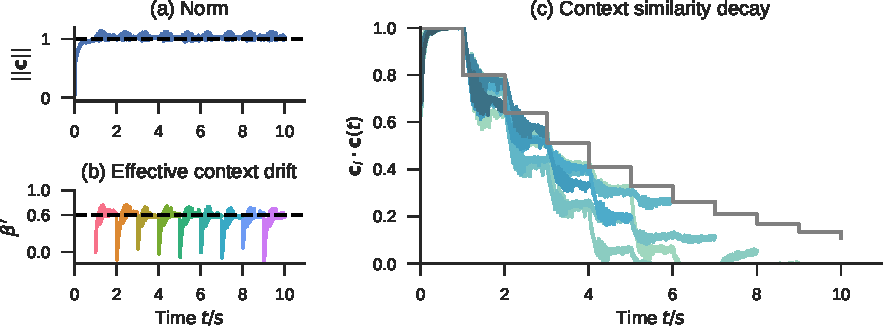
\includegraphics{bounded-integrator-orthogonal}
    \caption{
        Properties of the context vectors produces by the bounded integrator context network.
        It was provided with a new input context vector every second.
        Upper left: \ltwo-norm of the context.
        Lower left: Similarity of the context to the new input context.
        Right: The blue lines show the similarity of the context after each update to future context vectors.
        The red shading shows the expected similarities for different values of $\tcmbeta$ with the darkest shading corresponding to the target of $\tcmbeta = 0.6$.}\label{fig:bounded-integrator-orthogonal}
\end{figure}
\begin{figure}
    \centering
    \includegraphics{boundint}
    \caption{
        Properties of the context vectors produces by the bounded integrator context network.
        It was provided with a new input context vector every second.
        Upper left: \ltwo-norm of the context.
        Lower left: Similarity of the context to the new input context.
        Right: The blue lines show the similarity of the context after each update to future context vectors.
        The red shading shows the expected similarities for different values of $\tcmbeta$ with the darkest shading corresponding to the target of $\tcmbeta = 0.6$.}\label{fig:boundint}
\end{figure}

\section{Alternating update of two memories}
With a single integrator we have to rely on the dot product between the input vector and current context as a measure of $\tcmbeta$.
To circumvent this we need to use to gated memory populations that are updated in alternating fashion.
Then the output of the old context and input vector can be combined according to $\rho \ctx + \tcmbeta \ctxin$ and fed into to the memory buffer for the current context.
The completion of that memory update can be detected by the dot product of the updated context and the current context crossing 1.
\begin{figure}
    \centering
    \begin{tikzpicture}[nef, x=2cm, y=2cm]
        \graph [no placement] {
            in/\ctxin [ext, at={(0,0)}] -> ["$\tcmbeta$"] new/ [pnode, at={(1,0)}] -> cgate/ [ea, at={(2, 1)}] -> current/\ctx [ea, at={(3, 1)}] -> oldgate/ [ea, at={(3, -1)}] -> old/$\ctx'$ [ea, at={(2, -1)}] -> ["$\rho$"] new,
            current -> [bend right, "$-1$"] cgate,
            new -> [out=0, in=225] dot [net, at={(4, 1)}], current -> dot [net],
            dot -> rectification/ [rect, at={(4.5, 0.5)}] -> ["$\Heavi(x)$" anchor=west] heavi/ [pnode, at={(4.5, -0.5)}] -> [inhibit, bend left] cgate,
            heavi -> [inhibit] invert/ [ens, at={(4, -1)}] -> [inhibit] oldgate,
            bias/1 [ext, at={(4.5, -1)}] -> invert,
            old -> [bend right, "$-1$" below] oldgate
        };
    \end{tikzpicture}
    \caption{Alternating update of memory buffers.}\label{fig:ctx-bounded-integrator}
\end{figure}

Unfortunately, this still does not work for input vectors with some similarity.
In that case the dot product of the updated context and current context will already be quite high and the updated context is not completely loaded into the current memory buffer.
\begin{figure}
    \centering
    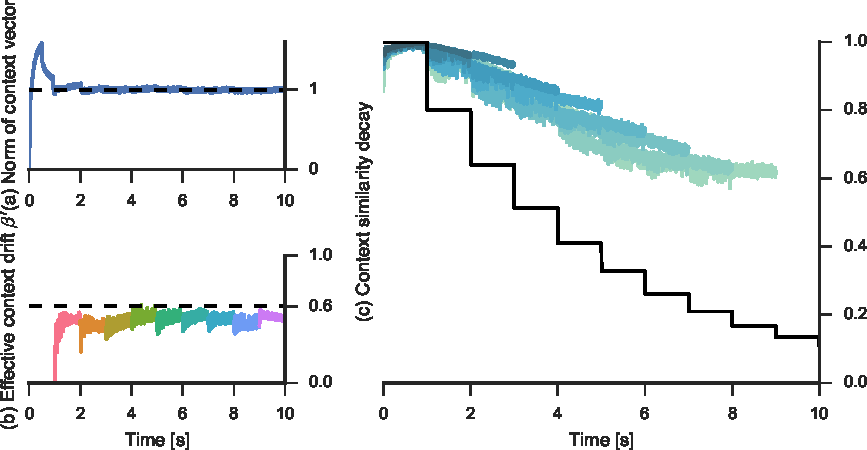
\includegraphics{alternating-memory-buffers}
    \caption{
        Properties of the context vectors produces by the alternating update of two memories context network.
        It was provided with a new input context vector every second with a similarity of approximately $\sqrt{1. - \beta^2}$ between consecutive vectors.
        Upper left: \ltwo-norm of the context.
        Lower left: Similarity of the context to the new input context.
        Right: The blue lines show the similarity of the context after each update to future context vectors.
        The red shading shows the expected similarities for different values of $\tcmbeta$ with the darkest shading corresponding to the target of $\tcmbeta = 0.6$.}\label{fig:alternating-memory-buffers}
\end{figure}


\section{Externally controlled alternating memory buffers}
All approaches to determine required context updates based on vector similarity will fail because the similarity of $\ctxin_i$ and $\ctx_{i-1}$ is not known beforehand and can vary widely depending on what contexts are recalled.
Thus, for a properly working context update in the TCM model, the update process has to be controlled by an external control signal (TODO reference other chapter).
If we take the alternating memory buffer network, it works for both orthogonal and similar input vectors.
\begin{figure}
    \centering
    \begin{tikzpicture}[nef, x=2cm, y=2cm]
        \graph [no placement] {
            in/\ctxin [ext, at={(0,0.5)}] -> ["$\tcmbeta$"] new/ [pnode, at={(1,0.5)}] -> cgate/ [ea, at={(2, 1)}] -> current/\ctx [ea, at={(3,1)}] -> oldgate/ [ea, at={(3, -1)}] -> old/$\ctx'$ [ea, at={(2, -1)}] -> ["$\rho$" {very near start, below}] new,
            current -> [bend right, "$-1$"] cgate,
            TODO [ext, at={(0,-.5)}] -> ctrl/ [pnode, at={(1,-.5)}] -> [inhibit] cgate,
            ctrl -> ["$-1$" near end] invert/ [pnode, at={(2.5, -0.5)}] -> [inhibit] oldgate,
            bias/1 [ext, at={(2.5, 0)}] -> invert,
            old -> [bend right, "$-1$" below] oldgate
        };
    \end{tikzpicture}
    \caption{Alternating update of memory buffers.}\label{fig:ctx-bounded-integrator}
\end{figure}

This leads to a number of predictions.
First, the update of the context signal is not directly regulated by the input, but externally controlled.
Second, there are neural populations that will start representing the current context in succession.
